\documentclass{IEEEtran}

\usepackage{graphicx}
\usepackage{subfig}
\usepackage{verbatim}
\usepackage{url}
\usepackage{listings}
\usepackage[utf8x]{inputenc}
\usepackage{float}
\usepackage{array}
\usepackage{booktabs}
\usepackage{tikz}
\usepackage{natbib}
\usepackage{algorithm}% http://ctan.org/pkg/algorithms
\usepackage{algpseudocode}% http://ctan.org/pkg/algorithmicx
\usepackage{xcolor,colortbl}
\usetikzlibrary{shapes,arrows,calc,shapes.multipart,positioning}
\usepackage{amsmath,amsfonts,amsthm} % Math packages
\usepackage{listings}
\usepackage{longtable}

\lstloadlanguages{Matlab}%
\lstset{language=Matlab,                        % Use MATLAB
        frame=single,                           % Single frame around code
        basicstyle=\scriptsize\ttfamily,        % Use small true type font
        keywordstyle=[1]\color{blue}\bfseries,  % MATLAB functions bold and blue
        keywordstyle=[2]\color{purple},         % MATLAB function arguments purple
        keywordstyle=[3]\color{blue}\underbar,  % User functions underlined and blue
        identifierstyle=,                        % Nothing special about identifiers
                                                % Comments small dark green courier
        commentstyle=\usefont{T1}{pcr}{m}{sl}\color{MyDarkGreen}\small,
        stringstyle=\color{purple},             % Strings are purple
        showstringspaces=false,                 % Don't put marks in string spaces
        tabsize=5,                              % 5 spaces per tab
        %
        %%% Put standard MATLAB functions not included in the default
        %%% language here
        morekeywords={xlim,ylim,var,alpha,factorial,poissrnd,normpdf,normcdf},
        %
        %%% Put MATLAB function parameters here
        morekeywords=[2]{on, off, interp},
        %
        %%% Put user defined functions here
        morekeywords=[3]{FindESS, homework_example},
        %
        morecomment=[l][\color{blue}]{...},     % Line continuation (...) like blue comment
        numbers=left,                           % Line numbers on left
        firstnumber=1,                           % Line numbers start with line 1
        numberstyle=\tiny\color{blue},          % Line numbers are blue
        stepnumber=1                            % Line numbers go in steps of 5
        }

\begin{document}

\title{Image Characterisation using Texture}
\date {March 2014}
\author{\IEEEauthorblockN{Tatiana Lopez Guevara , Elizabeth Vargas Vargas\\}
\IEEEauthorblockA{University of Girona\\
tatiana@sirius.utp.edu.co, liz2102@gmail.com }}
\maketitle

\begin{abstract}
Segmentation and classification are well known unsupervised and supervised problems in artificial vision. This document review both of them based on texture feature extracted using co-ocurrence matrices. The pertinence of the features is evaluated in a set of test images and the results are presented. Depending on the characteristics of each image different features are used, in order to improve segmentation accuracy and number of correct classified images.
\end{abstract}

\begin{IEEEkeywords}
Segmentation, region growing, classification
\end{IEEEkeywords}

\section{Introduction}

Segmentation is a well known unsupervised problem in the image processing field given
it's multiple application areas, such as medicine, object recognition, etc.
Different strategies has been proposed in order to solve it. However, there is
not an absolute answer for the problem, given that the obtained results depends
on the parameters used and on the nature of the image.\\

Classification on the other hand, is a supervised problem, where a set of elements should be correctly organized in classes previously defined. The problem has main applications in artificial vision, specially for object recognition.\\

\section{Problem Definition}

The segmentation problem tries to divide an image in different regions, such
that objects belonging to the region do not overlap and the union is the entire image. The regions should follow a set of rules, in order to
accept the segmentation as appropriate. These rules include uniformity,
simple interiors without holes and spatially accurate separation.\\

The problem consists in determining a quantitative way to decide whether a
segmentation is meaningful or not, depending on the application field. The
approaches followed in the literature use different elements such as
pre-processing techniques or determined parameters according to the 
type of image that need to be segmented. \cite{haralick1985image}\\

Classification deals with organizing objects in different groups, that has already been labelled according to a determined criteria. The challenge of classification is to determine the appropriate features that allows the differentiation of objects that belongs to different classes and the choose of a classifier that is able to detect those differences.

\section{Implementation}

\subsection{Co-ocurrence Matrices}

Co-ocurrence matrices were used in order to extract texture features from images, used to perform further segmentation and classification. Figure \ref{code:co_matrix} presents the used of the MATLAB functions that implements these kind of matrices. 

\begin{figure}[h!]
\begin{lstlisting}
im = rgb2gray(im);
comat_im = graycomatrix(im, 'Offset',[0 2], 
						'Symmetric', true);
stats_im = graycoprops(comat_im,{'Contrast','Homogeneity', 
						'Energy', 'Correlation'});
stats_im = struct2array( stats_im );
\end{lstlisting} 
 \caption{Co-ocurrence matrix}
 \label{code:co_matrix}
\end{figure}

The function 

\subsection{Segmentation}

% normalization

The region growing pseudocode is presented in Algorithm \ref{alg:rg}. The general 
implementation will be explained for gray scale images, given that in
color images the procedure is the same, with the addition of two channels,
$RGB$.\\

In color images, for each $RGB$ channel the statistics are saved. The agregation
function is computed by using the following formula:

\begin{equation}
\sqrt{(R - R_{\mu})^2 + (G - G_{\mu})^2 + (B - B_{\mu})^2} < threshold
\end{equation}

\subsection{Classification}

A set of 20 different classes of images were classified using the Random Forest classifier provided by the data mining tool WEKA. For each class, a set of six images were provided, with labels $1$, $5$, $9$, $13$, $17$ and $21$. Images with labels $1$ and $5$ were used as a training for the classifier and the rest were used for testing. The implementation consisted in determining a set of features from each image, in order to improve the accuracy of the classification. The proposed features were the following:

\begin{itemize}
 \item \textbf{Gray channel mean:} The image was transformed into a gray representation, (in case we were dealing with a color image) and the mean value was computed.
 \item \textbf{Texture features (CHECorr):} Using a global co-ocurrence matrix, in orientation $0^{\circ}$, distance 2 and the statistics Contrast, Homogeneity, Enery and Correlation, a set of texture features of the image were computed, using the matlab functions \texttt{graycomatrix} and \texttt{graycoprops}.
 \item \textbf{Texture features (CH):} It is a simplied version of the previous set of features, where only Contrast and Homogeneity are considered.
 \item \textbf{RGB mean:} The images that were using for classification were analysed, in order to determine by visual inspection which kind of features are the most representative for each image. The conclusion was that the color is the characteristic that is easier to differentiate between different sets. Table \ref{tb:color_features} presents the summarize of the color features from each set. 
 
\begin{table}[h!] 
\centering
\begin{tabular}{|c|c|c|c|}
\hline
\textbf{Set} & \textbf{Color} & \textbf{Set} & \textbf{Color} \\
\hline
t1 & \cellcolor{yellow!100}yellow & t11 & \cellcolor{green!25}light green \\
\hline
t2 & white & t12 & \cellcolor{brown!60}reddish brown \\
\hline
t3 & \cellcolor{green!50}green & t13 & \cellcolor{yellow!50}light yellow \\
\hline
t4 & \cellcolor{yellow!25}beige & t14 & \cellcolor{yellow!50}light yellow\\
\hline
t5 & \cellcolor{blue!100}blue & t15 & \cellcolor{yellow!25}beige \\
\hline
t6 & \cellcolor{purple!50}purple & t16 & \cellcolor{red!100}red \\
\hline
t7 & \cellcolor{blue!100}blue & t17 & white \\
\hline
t8 & \cellcolor{brown!100}brown & t18 & \cellcolor{green!100}green \\
\hline
t9 & white & t19 & white\\
\hline
t10 & \cellcolor{blue!25}light blue & t20 & \cellcolor{brown!100}brown\\
\hline
\end{tabular}
\caption{Color features}
\label{tb:color_features}
\end{table} 
 
 \item \textbf{RGB mean \& Texture features:} This feature is the combination of the two type of features previously computed. 
 \item \textbf{CIELab mean:} The $RGB$ image were transform into the \textit{CIELab} color space, given that euclidean distance in that color space presents in general better results as comparison measurement than in other colors spaces. 
 \item \textbf{CIELab mean \& Texture features:} This feature is the combination of two type of features previously computed: textures using co-ocurrence matrices and the mean value of each channel in the CIELab color space.
\end{itemize}

\section{Experimental Results}

\subsection{Co-ocurrence Matrices Performance}

The system described in Table \ref{tb:hwoverview} was used to run the performance tests.\\

\begin{table}[h!] 
\centering
\begin{tabular}{|c|}
\hline
Hardware Overview:\\
\hline
  Model Name:   MacBook Pro\\
  Model Identifier: MacBookPro10,1\\
  Processor Name:   Intel Core i7\\
  Processor Speed:  2.3 GHz\\
  Number of Processors: 1\\ 
  Total Number of Cores:    4\\ 
  L2 Cache (per Core):  256 KB\\
  L3 Cache: 6 MB\\
  Memory:   8 GB\\
\hline
\end{tabular}
\caption{Hardware Overview}
\label{tb:hwoverview}
\end{table}

Table \ref{tb:performance} presents the time table with the execution time of the
algorithm that extracts statistics, according to the image used and the parameters used to compute them.

\begin{table}[h!]
\centering
\begin{tabular}{|c|c|c|c|c|c|}
\hline
Image & Size &\# Ang. & Dist. & \# Statistics & Time \\  
\hline
Feli & 382 x 265 & 0 & 2 & 3 & 160.374 \\
\hline
Feli & 382 x 265  & 2 & 3 & 3 & 280.554 \\
\hline
Hand & 288 x 228 & 1 & 3 & 3 & 141.983 \\
\hline
Hand & 288 x 228 & 4 & 1 & 3 & 151.944\\
\hline
\end{tabular}
\caption{Texture Feature Extraction Execution Time}
\label{tb:performance}
\end{table} 

\subsection{Segmentation Results}

The segmentation results obtained for different images are presented individually in this section, given that for each image in particular, the parameters were determined by analysing the characteristics of the image. In each case, a comparison between the segmented image using colors and textures is presented, in order to evaluate the pertinence or not of the features.\\

\begin{table}[h!] 
\centering
\begin{tabular}{|c|}
\hline
Feli Texture Features:\\
\hline
  Gray Levels:   8\\
  Window Size: 13\\
  Distance:   [1 2]\\
  Orientation:  $45^{\circ}$, $135^{\circ}$\\
\hline
\end{tabular}
\caption{Feli texture features parameters}
\label{tb:param_feli}
\end{table}

The textures features from \textit{Feli} were extracted using the parameters of the Table \ref{tb:param_feli}. The parameters were determining by observing the different images generated from different features, in order to identify which one presents the most notable differences between regions. Figures \ref{fig:feli_45} and \ref{fig:feli_135} presents the features contrast, homogeneity and energy for the orientations $45^{\circ}$ and $135^{\circ}$ respectively. As can be seen in the images, the difference between the background and foreground is remarkable, making these kind of features useful for performing a meaningful segmentation.\\

\begin{figure}[h!] 
 \centering
 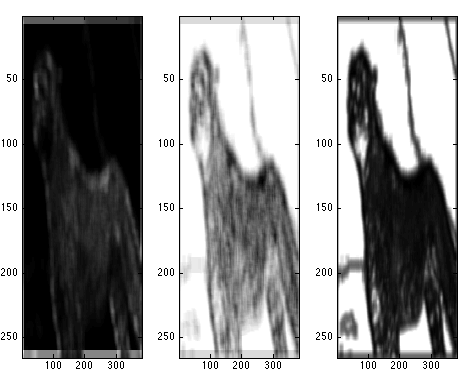
\includegraphics[width=175pt,height=75pt]{./fig/feli/fstats_135_n1_1.png}%
 \caption{Statistics using $45^{\circ}$}
 \label{fig:feli_45}
\end{figure}

\begin{figure}[h!] 
 \centering
 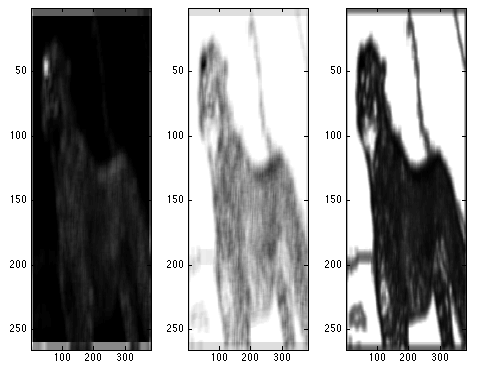
\includegraphics[width=175pt,height=75pt]{./fig/feli/fstats_135_n1_n1.png}%
 \caption{Statistics using $135^{\circ}$}
 \label{fig:feli_135}
\end{figure}

Figure \ref{fig:feli_seg} presents the results obtained when segmenting the image using color features (left) and color combined with texture features (right). The threshold value used for color segmentation was $40$, while for the combined feature vector was $58$. By visual inspection can be verified that the image on the left side is oversegmented, given that the animal appears in different regions. On the other hand, the right image presents a clear different between background and foreground and the silhouette of the animal can be easily recognized.

\begin{figure}[h!] 
 \centering
 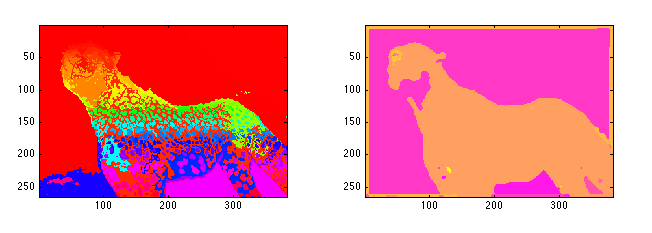
\includegraphics[width=250pt]{./fig/feli/fres_all_58.png}%
 \caption{Segmentation results using color and texture features}
 \label{fig:feli_seg}
\end{figure}

\begin{table}[h!] 
\centering
\begin{tabular}{|c|}
\hline
Feli Texture Features:\\
\hline
  Gray Levels:   8\\
  Window Size: 15\\
  Distance:   1 \\
  Orientation: $135^{\circ}$\\
\hline
\end{tabular}
\caption{Hand texture features parameters}
\label{tb:param_feli}
\end{table}


\begin{figure}[h!] 
 \centering
 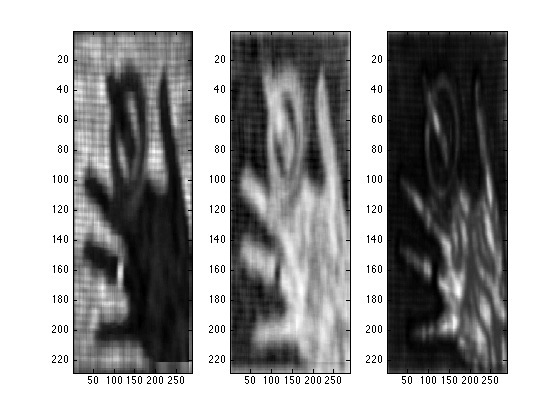
\includegraphics[width=175pt,height=75pt]{./fig/hand/fstats_1_135_end_5.png}%
 \caption{Statistics using $135^{\circ}$}
 \label{fig:feli_135}
\end{figure}

% threshold seg: 2.8015 ... RGB -> 65

\begin{figure}[h!] 
 \centering
 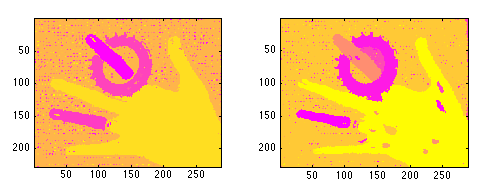
\includegraphics[width=250pt]{./fig/hand/res_1_all_w15_end_5.png}%
 \caption{Segmentation results using color and texture features}
 \label{fig:feli_seg}
\end{figure}

\subsection{Classification Accuracy}

Table \ref{tb:accuracy_class} presents the percentage of images that were correctly classified for each of the features extraction approaches previously presented.\\

% summary classification

\begin{table}[h!] 
\centering
\begin{tabular}{|c|c|}
\hline
\textbf{Strategy} & \textbf{Correct Classified (\%)} \\
\hline
Gray channel mean & 66.25  \\
\hline
Texture features (CHECorr) & 47.50  \\ % normalizing
\hline
Texture features (CH) & 63.75  \\ % without normalizing!, using only C = 42.5; H = 11.25
\hline
RGB mean & 93.75 \\
\hline
RGB mean \& Texture features & 100 \\ % al revés da: 87.50
\hline
CIELab mean & 95.00  \\
\hline
CIELab mean \& Texture features & 95.00  \\
\hline
\end{tabular}
\caption{Classification accuracy}
\label{tb:accuracy_class}
\end{table}

% TODO: describir el problema del RGB con respecto a las metricas: mean por ej.

The gray channel, which is the naive approach, turns in a percentage of images that are correctly classified of 66.25\%. When using normalized texture features however, the percentage decreased to 47.50\%. This can be explained given the orientation used, given that was calculated only in one direction, and it is maybe not the most representative direction for all the set of images. In a further test, only the first two statistics were used, obtaining a result of correctly classified images of 63.75\%. Additional tests showed that using only contrast did not lead to a good result (42.5\%) and neither homogeneity (11.25\%). So it means, that is the combination of both statistics, without normalization, that leads to a good result. A better result was obtained when the mean of the $RGB$ values was used, 93.75\%. It can be explained because the most prominent feature of the set of images is color, given that each image has only one type of object. The best result is obtained when the $RGB$ mean is combined with texture features. In that case, the obtained result is 100\% of images correctly classified. In this part, the experiment of changing the order of the feature vector was made, but the result was not the same one: 87.5\%. At last, the color space was changed, in order to use CIELab and the mean of each channel was used as a feature. The result of applying the classification algorithm using those features is 95\%. Adding the texture features to that vector does not change the result, as can be seen on the table. So we can say that the texture features only improves the accuracy on the $RGB$ color space, but in $CIELab$ it has no positive or negative effect.\\


On the appendix, the most relevant confusion matrices are presented with the diagonal highlighted (representing the images that are correctly classified). Table \ref{tb:rgb_texture} presents the matrix where all the images has been correctly classified. It can be seen that in that matrix, there are values only in the diagonal. The feature that leads to this classification is the \textbf{RGB mean \& Texture features}

\section{Organization of Coursework}

In order to organize the tasks to develop as well as the version control of the code,
the tool {\bf github} was used. The repository of this project can be find at:
\textit{https://github.com/ZePoLiTaT/SegmentationUsingTexture}.\\

The distribution of the work per person is presented in Table \ref{table:time}.

\begin{table}[h!]
\centering
  \begin{tabular}{ | c | c | }
    \hline
    Activity & Time (hours)  \\ \hline
    Laboratory & 4\\ \hline
    Implementation & 6 \\ \hline
    Test & 8 \\ \hline
    Report & 6 \\ \hline
    TOTAL & 24 \\ \hline
  \end{tabular}
  \caption{Time distribution}
  \label{table:time}
\end{table}

\section{Conclusions and Future Work}

\begin{itemize}
 \item The features used in order to perform a proper classification relies mostly on the nature of the image. It could be appreciated in the classification exercise, when the use of color features increased the percentage of images correctly classified in around 40\%. 
 \item The order in which the features are used in the vector had an impact on the Random Forest Tree classifier, given that for different order of the features inside the vector, the obtained result was different. A future work in this area is the use of another classifier.
\end{itemize}

\bibliographystyle{plain}
\bibliography{biblio}

\newpage
\onecolumn
\appendix

% gray mean

\begin{table}[h!]
\centering
\begin{tabular}{|c|c|c|c|c|c|c|c|c|c|c|c|c|c|c|c|c|c|c|c|}
\hline
\textbf{t1} & \textbf{t2} & \textbf{t3} & \textbf{t4} & \textbf{t5} & \textbf{t6} & \textbf{t7} & \textbf{t8} & \textbf{t9} & \textbf{t10} & \textbf{t11} & \textbf{t12} &
\textbf{t13} & \textbf{t14} & \textbf{t15} & \textbf{t16} & \textbf{t17} & \textbf{t18} &
\textbf{t19} & \textbf{t20} \\
\hline
\cellcolor{green!40}2 & 0 & \cellcolor{red!25}1 & 0 & \cellcolor{red!25}1 & 0 & 0 & 0 & 0 & 0 & 0 & 0 & 0 & 0 & 0 & 0 & 0 & 0 & 0 & 0\\
\hline
0 & \cellcolor{green!40}1 & 0 & 0 & 0 & 0 & 0 & 0 & 0 & 0 & \cellcolor{red!25}1 & \cellcolor{red!25}2 & 0 & 0 & 0 & 0 & 0 & 0 & 0 & 0\\
\hline
2 & 0 & \cellcolor{green!40}1 & 0 & 0 & 0 & 0 & 0 & 0 & 0 & 0 & 0 & 0 & 0 & 0 & 0 & \cellcolor{red!25}1 & 0 & 0 & 0\\
\hline
0 & 0 & 0 & \cellcolor{green!40}4 & 0 & 0 & 0 & 0 & 0 & 0 & 0 & 0 & 0 & 0 & 0 & 0 & 0 & 0 & 0 & 0\\
\hline
0 & 0 & 0 & 0 & \cellcolor{green!40}4 & 0 & 0 & 0 & 0 & 0 & 0 & 0 & 0 & 0 & 0 & 0 & 0 & 0 & 0 & 0\\
\hline
0 & 0 & 0 & 0 & 0 & \cellcolor{green!40}4 & 0 & 0 & 0 & 0 & 0 & 0 & 0 & 0 & 0 & 0 & 0 & 0 & 0 & 0\\
\hline
0 & 0 & 0 & 0 & 0 & \cellcolor{red!25}3 & \cellcolor{green!40}0 & 0 & 0 & \cellcolor{red!25}1 & 0 & 0 & 0 & 0 & 0 & 0 & 0 & 0 & 0 & 0\\
\hline
0 & 0 & 0 & 0 & 0 & 0 & 0 & \cellcolor{green!40}4 & 0 & 0 & 0 & 0 & 0 & 0 & 0 & 0 & 0 & 0 & 0 & 0\\
\hline
0 & \cellcolor{red!25}1 & 0 & 0 & 0 & 0 & 0 & 0 & \cellcolor{green!40}2 & 0 & \cellcolor{red!25}1 & 0 & 0 & 0 & 0 & 0 & 0 & 0 & 0 & 0\\
\hline
0 & 0 & 0 & 0 & 0 & \cellcolor{red!25}1 & 0 & 0 & 0 & \cellcolor{green!40}3 & 0 & 0 & 0 & 0 & 0 & 0 & 0 & 0 & 0 & 0\\
\hline
0 & \cellcolor{red!25}2 & 0 & 0 & 0 & 0 & 0 & 0 & 0 & 0 & \cellcolor{green!40}2 & 0 & 0 & 0 & 0 & 0 & 0 & 0 & 0 & 0\\
\hline
0 & 0 & 0 & 0 & 0 & 0 & 0 & 0 & 0 & 0 & 0 & \cellcolor{green!40}4 & 0 & 0 & 0 & 0 & 0 & 0 & 0 & 0\\
\hline
0 & 0 & 0 & 0 & 0 & 0 & 0 & 0 & 0 & 0 & 0 & 0 & \cellcolor{green!40}4 & 0 & 0 & 0 & 0 & 0 & 0 & 0\\
\hline
0 & 0 & 0 & 0 & 0 & 0 & 0 & 0 & 0 & 0 & 0 & 0 & 2 & \cellcolor{green!40}2 & 0 & 0 & 0 & 0 & 0 & 0\\
\hline
0 & 0 & 0 & 0 & 0 & 0 & 0 & 0 & \cellcolor{red!25}2 & 0 & 0 & 0 & 0 & 0 & \cellcolor{green!40}2 & 0 & 0 & 0 & 0 & 0\\
\hline
0 & 0 & 0 & 0 & 0 & 0 & 0 & 0 & 0 & 0 & 0 & 0 & 0 & 0 & 0 & \cellcolor{green!40}3 & 0 & \cellcolor{red!25}1 & 0 & 0\\
\hline
0 & 0 & \cellcolor{red!25}3 & 0 & 0 & 0 & 0 & 0 & 0 & 0 & 0 & 0 & 0 & 0 & 0 & 0 & \cellcolor{green!40}1 & 0 & 0 & 0\\
\hline
0 & 0 & 0 & 0 & 0 & 0 & 0 & 0 & 0 & \cellcolor{red!25}2 & 0 & 0 & 0 & 0 & 0 & 0 & 0 & \cellcolor{green!40}2 & 0 & 0\\
\hline
0 & 0 & 0 & 0 & 0 & 0 & 0 & 0 & 0 & 0 & 0 & 0 & 0 & 0 & 0 & 0 & 0 & 0 & \cellcolor{green!40}4 & 0\\
\hline
0 & 0 & 0 & 0 & 0 & 0 & 0 & 0 & 0 & 0 & 0 & 0 & 0 & 0 & 0 & 0 & 0 & 0 & 0 & \cellcolor{green!40}4\\
\hline
\end{tabular}
\caption{Gray channel mean}
\label{tb:gray_mean}
\end{table}

% RGB mean

\begin{table}[h!]
\centering
\begin{tabular}{|c|c|c|c|c|c|c|c|c|c|c|c|c|c|c|c|c|c|c|c|}
\hline
\textbf{t1} & \textbf{t2} & \textbf{t3} & \textbf{t4} & \textbf{t5} & \textbf{t6} & \textbf{t7} & \textbf{t8} & \textbf{t9} & \textbf{t10} & \textbf{t11} & \textbf{t12} &
\textbf{t13} & \textbf{t14} & \textbf{t15} & \textbf{t16} & \textbf{t17} & \textbf{t18} &
\textbf{t19} & \textbf{t20} \\
\hline
\cellcolor{blue!25}4 & 0 & 0 & 0 & 0 & 0 & 0 & 0 & 0 & 0 & 0 & 0 & 0 & 0 & 0 & 0 & 0 & 0 & 0 & 0\\
\hline
0 & \cellcolor{blue!25}4 & 0 & 0 & 0 & 0 & 0 & 0 & 0 & 0 & 0 & 0 & 0 & 0 & 0 & 0 & 0 & 0 & 0 & 0\\
\hline
0 & 0 & \cellcolor{blue!25}4 & 0 & 0 & 0 & 0 & 0 & 0 & 0 & 0 & 0 & 0 & 0 & 0 & 0 & 0 & 0 & 0 & 0\\
\hline
0 & 0 & 0 & \cellcolor{blue!25}4 & 0 & 0 & 0 & 0 & 0 & 0 & 0 & 0 & 0 & 0 & 0 & 0 & 0 & 0 & 0 & 0\\
\hline
0 & 0 & 0 & 0 & \cellcolor{blue!25}4 & 0 & 0 & 0 & 0 & 0 & 0 & 0 & 0 & 0 & 0 & 0 & 0 & 0 & 0 & 0\\
\hline
0 & 0 & 0 & 0 & 0 & \cellcolor{blue!25}4 & 0 & 0 & 0 & 0 & 0 & 0 & 0 & 0 & 0 & 0 & 0 & 0 & 0 & 0\\
\hline
0 & 0 & 0 & 0 & 0 & 0 & \cellcolor{blue!25}4 & 0 & 0 & 0 & 0 & 0 & 0 & 0 & 0 & 0 & 0 & 0 & 0 & 0\\
\hline
0 & 0 & 0 & 0 & 0 & 0 & 0 & \cellcolor{blue!25}2 & 0 & \cellcolor{red!25}1 & 0 & 0 & 0 & 0 & 0 & 0 & 0 & 0 & \cellcolor{red!25}1 & 0\\
\hline
0 & 0 & 0 & 0 & 0 & 0 & 0 & 0 & \cellcolor{blue!25}4 & 0 & 0 & 0 & 0 & 0 & 0 & 0 & 0 & 0 & 0 & 0\\
\hline
0 & 0 & 0 & 0 & 0 & 0 & 0 & 0 & 0 & \cellcolor{blue!25}3 & 0 & 0 & 0 & 0 & 0 & 0 & \cellcolor{red!25}1 & 0 & 0 & 0\\
\hline
0 & 0 & 0 & 0 & 0 & 0 & 0 & 0 & 0 & 0 & \cellcolor{blue!25}4 & 0 & 0 & 0 & 0 & 0 & 0 & 0 & 0 & 0\\
\hline
0 & 0 & 0 & 0 & 0 & 0 & 0 & 0 & 0 & 0 & 0 & \cellcolor{blue!25}4 & 0 & 0 & 0 & 0 & 0 & 0 & 0 & 0\\
\hline
0 & 0 & 0 & 0 & 0 & 0 & 0 & 0 & 0 & 0 & 0 & 0 & \cellcolor{blue!25}4 & 0 & 0 & 0 & 0 & 0 & 0 & 0\\
\hline
0 & 0 & 0 & 0 & 0 & 0 & 0 & 0 & 0 & 0 & 0 & 0 & 0 & \cellcolor{blue!25}4 & 0 & 0 & 0 & 0 & 0 & 0\\
\hline
0 & 0 & 0 & 0 & \cellcolor{red!25}1 & 0 & 0 & 0 & 0 & 0 & 0 & 0 & 0 & 0 & \cellcolor{blue!25}3 & 0 & 0 & 0 & 0 & 0\\
\hline
0 & 0 & 0 & 0 & 0 & 0 & 0 & 0 & 0 & 0 & 0 & 0 & 0 & 0 & 0 & \cellcolor{blue!25}4 & 0 & 0 & 0 & 0\\
\hline
0 & 0 & 0 & 0 & 0 & 0 & 0 & 0 & 0 & 0 & 0 & 0 & 0 & 0 & 0 & 0 & \cellcolor{blue!25}4 & 0 & 0 & 0\\
\hline
0 & 0 & 0 & 0 & 0 & 0 & 0 & 0 & 0 & 0 & 0 & 0 & 0 & 0 & 0 & 0 & 0 & \cellcolor{blue!25}4 & 0 & 0\\
\hline
0 & 0 & 0 & 0 & 0 & 0 & 0 & 0 & 0 & \cellcolor{red!25}1 & 0 & 0 & 0 & 0 & 0 & 0 & 0 & 0 & \cellcolor{blue!25}3 & 0\\
\hline
0 & 0 & 0 & 0 & 0 & 0 & 0 & 0 & 0 & 0 & 0 & 0 & 0 & 0 & 0 & 0 & 0 & 0 & 0 & \cellcolor{blue!25}4\\
\hline
\end{tabular}
\caption{RGB mean}
\label{tb:rgb_mean}
\end{table}

\begin{table}[h!] 
\centering
\begin{tabular}{|c|c|c|c|c|c|c|c|c|c|c|c|c|c|c|c|c|c|c|c|}
\hline
\textbf{t1} & \textbf{t2} & \textbf{t3} & \textbf{t4} & \textbf{t5} & \textbf{t6} & \textbf{t7} & \textbf{t8} & \textbf{t9} & \textbf{t10} & \textbf{t11} & \textbf{t12} &
\textbf{t13} & \textbf{t14} & \textbf{t15} & \textbf{t16} & \textbf{t17} & \textbf{t18} &\textbf{t19} & \textbf{t20} \\
\hline
\cellcolor{purple!30}4 & 0 & 0 & 0 & 0 & 0 & 0 & 0 & 0 & 0 & 0 & 0 & 0 & 0 & 0 & 0 & 0 & 0 & 0 & 0\\
\hline
0 & \cellcolor{purple!30}4 & 0 & 0 & 0 & 0 & 0 & 0 & 0 & 0 & 0 & 0 & 0 & 0 & 0 & 0 & 0 & 0 & 0 & 0\\
\hline
0 & 0 & \cellcolor{purple!30}4 & 0 & 0 & 0 & 0 & 0 & 0 & 0 & 0 & 0 & 0 & 0 & 0 & 0 & 0 & 0 & 0 & 0\\
\hline
0 & 0 & 0 & \cellcolor{purple!30}4 & 0 & 0 & 0 & 0 & 0 & 0 & 0 & 0 & 0 & 0 & 0 & 0 & 0 & 0 & 0 & 0\\
\hline
0 & 0 & 0 & 0 & \cellcolor{purple!30}4 & 0 & 0 & 0 & 0 & 0 & 0 & 0 & 0 & 0 & 0 & 0 & 0 & 0 & 0 & 0\\
\hline
0 & 0 & 0 & 0 & 0 & \cellcolor{purple!30}4 & 0 & 0 & 0 & 0 & 0 & 0 & 0 & 0 & 0 & 0 & 0 & 0 & 0 & 0\\
\hline
0 & 0 & 0 & 0 & 0 & 0 & \cellcolor{purple!30}4 & 0 & 0 & 0 & 0 & 0 & 0 & 0 & 0 & 0 & 0 & 0 & 0 & 0\\
\hline
0 & 0 & 0 & 0 & 0 & 0 & 0 & \cellcolor{purple!30}4 & 0 & 0 & 0 & 0 & 0 & 0 & 0 & 0 & 0 & 0 & 0 & 0\\
\hline
0 & 0 & 0 & 0 & 0 & 0 & 0 & 0 & \cellcolor{purple!30}4 & 0 & 0 & 0 & 0 & 0 & 0 & 0 & 0 & 0 & 0 & 0\\
\hline
0 & 0 & 0 & 0 & 0 & 0 & 0 & 0 & 0 & \cellcolor{purple!30}4 & 0 & 0 & 0 & 0 & 0 & 0 & 0 & 0 & 0 & 0\\
\hline
0 & 0 & 0 & 0 & 0 & 0 & 0 & 0 & 0 & 0 & \cellcolor{purple!30}4 & 0 & 0 & 0 & 0 & 0 & 0 & 0 & 0 & 0\\
\hline
0 & 0 & 0 & 0 & 0 & 0 & 0 & 0 & 0 & 0 & 0 & \cellcolor{purple!30}4 & 0 & 0 & 0 & 0 & 0 & 0 & 0 & 0\\
\hline
0 & 0 & 0 & 0 & 0 & 0 & 0 & 0 & 0 & 0 & 0 & 0 & \cellcolor{purple!30}4 & 0 & 0 & 0 & 0 & 0 & 0 & 0\\
\hline
0 & 0 & 0 & 0 & 0 & 0 & 0 & 0 & 0 & 0 & 0 & 0 & 0 & \cellcolor{purple!30}4 & 0 & 0 & 0 & 0 & 0 & 0\\
\hline
0 & 0 & 0 & 0 & 0 & 0 & 0 & 0 & 0 & 0 & 0 & 0 & 0 & 0 & \cellcolor{purple!30}4 & 0 & 0 & 0 & 0 & 0\\
\hline
0 & 0 & 0 & 0 & 0 & 0 & 0 & 0 & 0 & 0 & 0 & 0 & 0 & 0 & 0 & \cellcolor{purple!30}4 & 0 & 0 & 0 & 0\\
\hline
0 & 0 & 0 & 0 & 0 & 0 & 0 & 0 & 0 & 0 & 0 & 0 & 0 & 0 & 0 & 0 & \cellcolor{purple!30}4 & 0 & 0 & 0\\
\hline
0 & 0 & 0 & 0 & 0 & 0 & 0 & 0 & 0 & 0 & 0 & 0 & 0 & 0 & 0 & 0 & 0 & \cellcolor{purple!30}4 & 0 & 0\\
\hline
0 & 0 & 0 & 0 & 0 & 0 & 0 & 0 & 0 & 0 & 0 & 0 & 0 & 0 & 0 & 0 & 0 & 0 & \cellcolor{purple!30}4 & 0\\
\hline
0 & 0 & 0 & 0 & 0 & 0 & 0 & 0 & 0 & 0 & 0 & 0 & 0 & 0 & 0 & 0 & 0 & 0 & 0 & \cellcolor{purple!30}4\\
\hline
\end{tabular}
\caption{RGB mean \& Texture features}
\label{tb:rgb_texture}
\end{table}

\end{document}

